\section{Preliminaries: a table is a counting function}
\label{sec:prelim}

\subsection{The one idea everything rests on}

Write a bag not as a list of rows but as a function that counts:

\keybox{Definition you must internalise}{%
$R(t)$ = ``how many copies of the row $t$ are in table $R$?''\\[3pt]
A table of schema $\sigma$ is a function $\Tup{\sigma} \to \mathbb{N}$, where
$\Tup{\sigma}$ is the set of \emph{all} tuples of that schema --- not just the ones
present. Absent rows simply have count $0$.}

This is the \emph{$K$-relation} view of Green, Karvounarakis and Tannen~\cite{green}, with
$K = \mathbb{N}$. Running example throughout:

\begin{center}\small
\begin{tabular}{@{}ll@{}}
\begin{tabular}{@{}c|c@{}}
\multicolumn{2}{@{}l}{$R$}\\
\toprule
$x$ & $y$\\\midrule
1 & 10\\ 1 & 20\\ 2 & 30\\\bottomrule
\end{tabular}
&\hspace{12mm}
\begin{tabular}{@{}c|c@{}}
\multicolumn{2}{@{}l}{$S$ \small(primary key on $a$)}\\
\toprule
$a$ & $b$\\\midrule
1 & 100\\\bottomrule
\end{tabular}
\end{tabular}
\end{center}

\noindent so $R(1,10)=1$, $R(1,20)=1$, $R(2,30)=1$, and $R(t)=0$ for every other $t$;
$S(1,100)=1$ and $S(t)=0$ elsewhere. Verified:

\begin{lstlisting}[style=sql]
select count(*) from r where x = 1 and y = 10;   --> 1
select count(*) from r where x = 1 and y = 99;   --> 0
\end{lstlisting}

\subsection{Query operators as arithmetic}

Once tables are counting functions, the relational operators become arithmetic. This table
is the Rosetta stone for the whole document; each line is derived properly in
Section~\ref{sec:uexpr}.

\begin{table}[h]\centering\small
\begin{tabularx}{\linewidth}{@{}l l X@{}}
\toprule
\textbf{SQL} & \textbf{on counts} & \textbf{why} \\
\midrule
\lstinline|FROM R|                & $R(t)$ & by definition \\
\lstinline|WHERE b|               & $\ind{b}\times R(t)$ & $\ind{b}$ is $1$ or $0$; multiplying by $0$ deletes the row \\
\lstinline|R, S| (cross join)     & $R(t_1)\times S(t_2)$ & every left row pairs with every right row \\
\lstinline|UNION ALL|             & $R(t)+S(t)$ & copies accumulate \\
\lstinline|SELECT x| (projection) & $\usum{y} R(x,y)$ & forgetting $y$ merges rows, so counts add \\
\lstinline|DISTINCT|              & $\sq{R(t)}$ & clamp any count to $0$ or $1$ \\
\lstinline|NOT EXISTS Q|          & $\notu{\usum{t}Q(t)}$ & $1$ exactly when the count is $0$ \\
\bottomrule
\end{tabularx}
\caption{SQL as arithmetic on multiplicities.}
\label{tab:rosetta}
\end{table}

Two of these deserve immediate attention because beginners stumble on both.

\paragraph{Why projection is a sum.}
\lstinline|SELECT x FROM R| throws away $y$. Two rows that differed only in $y$ become the
same output row, so their counts must be \emph{added}:
\[
\den{\texttt{SELECT x FROM R}}(x) \;=\; \usum{y} R(x,y).
\]
Concretely $\usum{y}R(1,y) = 1+1 = 2$, which is exactly
\lstinline|SELECT x, count(*) FROM r GROUP BY x| returning $2$ for $x=1$.

\paragraph{Why the sum is ``unbounded''.}
The index $y$ ranges over \emph{every} value of its type, not over the rows of $R$. That
looks alarming --- an infinite sum --- but almost every term is $0$, because a table has
finitely many rows. Widening the range cannot change the value:

\begin{lstlisting}[style=sql]
select sum((select count(*) from r where r.x=1 and r.y=yv))
from generate_series(0,30) yv;        --> 2
-- same query over generate_series(-1000,1000)
                                      --> 2
\end{lstlisting}

Both \udp{} and \QED{} keep unbounded summation as a \emph{primitive} rather than proving
finiteness, because proving that every operator preserves finiteness is painful and buys
little~\cite[\S3.1]{udp}. \QED{} handles the pathological case by working in
$\Nbar=\mathbb{N}\cup\{\infty\}$ so that a genuinely infinite sum is still a well-defined
value.

\subsection{$\Sigma$ versus $\Sumagg$: two things called ``sum''}

This trips up almost everyone, so we fix it now.

\begin{table}[h]\centering\small
\begin{tabular}{@{}lllc@{}}
\toprule
 & \textbf{adds up} & \textbf{SQL} & \textbf{on the bag $\{10,20\}$} \\
\midrule
$\usum{y} f(y)$        & multiplicities            & \lstinline|COUNT(*)| & $1+1=2$ \\
$\Sumagg(\lam{y}{f(y)})$ & values $\times$ multiplicities & \lstinline|SUM(y)|   & $10{\cdot}1+20{\cdot}1=30$ \\
\bottomrule
\end{tabular}
\end{table}

\noindent Verified: \lstinline|select count(*), sum(y) from r where x = 1| returns
$2$ and $30$.

Here $\lam{y}{f(y)}$ is an anonymous function (Python's \texttt{lambda y:}). Because a bag
\emph{is} a counting function, writing $\lam{y}{R(1,y)}$ \emph{is} writing the bag
$\{10,20\}$. Aggregates consume a whole bag, so their argument must be a function, not a
number.

\subsection{The running example: aggregate pushdown through a join}
\label{sec:running}

Everything in this document is illustrated on one rewrite --- Calcite's
\texttt{AggregateJoinTransposeRule}, which is also \QED{}'s motivating example~\cite[\S2]{qed}.

\begin{lstlisting}[style=sql]
-- Q1 : aggregate ABOVE the join
select x, sum(y) as r from R join S on R.x = S.a group by x;

-- Q2 : aggregate BELOW the join
select t.x, t.r
from (select x, sum(y) as r from R group by x) t join S on t.x = S.a;
\end{lstlisting}

\subsubsection{Calcite plans (primary)}

These are real \texttt{RelNode} trees produced by Apache Calcite 1.19 with
\texttt{R(X,Y)} and \texttt{S(A,B)} declared, \texttt{S.A} unique
(\lstinline[style=pseudo]|Statistics.of(rows, ImmutableList.of(ImmutableBitSet.of(0)))|):

\begin{center}
\begin{minipage}{0.48\linewidth}
\begin{lstlisting}[style=plan]
-- Q1
LogicalAggregate(group=[{0}], SUMY=[SUM($1)])
  LogicalProject(X=[$0], Y=[$1])
    LogicalJoin(condition=[=($0,$2)],
                joinType=[inner])
      TableScan(table=[[R]])
      TableScan(table=[[S]])
\end{lstlisting}
\end{minipage}\hfill
\begin{minipage}{0.48\linewidth}
\begin{lstlisting}[style=plan]
-- Q2
LogicalProject(X=[$0], SUMY=[$1])
  LogicalJoin(condition=[=($0,$2)],
              joinType=[inner])
    LogicalAggregate(group=[{0}],
                     SUMY=[SUM($1)])
      TableScan(table=[[R]])
    TableScan(table=[[S]])
\end{lstlisting}
\end{minipage}
\end{center}

\noindent \texttt{LogicalAggregate} and \texttt{LogicalJoin} have swapped places. That is
the entire rewrite.

\subsubsection{Calcite applies the rule itself --- and reveals the key fact}
\label{sec:calcite-fires}

Running Calcite's own \texttt{AggregateJoinTransposeRule.EXTENDED} on $Q_1$ in a
\texttt{HepPlanner} gives two very different answers depending on whether \texttt{S.A} is
declared unique:

\begin{center}
\begin{minipage}{0.46\linewidth}
\centering\textbf{\small \texttt{S.A} declared unique}
\begin{lstlisting}[style=plan]
LogicalProject(X=[$0], SUMY=[$1])
  LogicalJoin(cond=[=($0,$2)])
    LogicalAggregate(group=[{0}],
                     SUMY=[SUM($1)])
      TableScan([[R]])
    LogicalProject(A=[$0])
      TableScan([[S]])
\end{lstlisting}
\smallskip
{\footnotesize\itshape exactly $Q_2$.}
\end{minipage}\hfill
\begin{minipage}{0.51\linewidth}
\centering\textbf{\small \texttt{S.A} \emph{not} unique}
\begin{lstlisting}[style=plan]
LogicalProject(X=[$0],
   $f4=[CAST(*($1, $3))])   <-- product!
  LogicalJoin(cond=[=($0,$2)])
    LogicalAggregate(group=[{0}],
                     SUMY=[SUM($1)])
      TableScan([[R]])
    LogicalAggregate(group=[{0}],
                 agg#0=[COUNT()])  <-- count!
      TableScan([[S]])
\end{lstlisting}
\smallskip
{\footnotesize\itshape \emph{not} $Q_2$: the aggregate is
multiplied by the number of matching \texttt{S} rows.}
\end{minipage}
\end{center}

\warnbox{Read this twice --- it is the whole document in one picture}{%
With the key, Calcite produces exactly $Q_2$. Without the key, Calcite \emph{refuses} to
produce $Q_2$; instead it counts the matching $S$ rows and \textbf{multiplies the
aggregate by that count}. That compensating factor is literally the $\times\,S(a)$ term of
the U-expression, discovered independently by a production optimiser. When we prove
$Q_1 \equiv Q_2$ in Sections \ref{sec:uexpr}--\ref{sec:lia}, the primary key is precisely
what lets us delete that factor.}

\subsubsection{PostgreSQL plans (secondary cross-check)}

PostgreSQL does \emph{not} attempt this rewrite, so the two SQL texts execute as written ---
which makes it a clean way to observe both shapes running. On $10^6$ rows in \texttt{r} and
$5\cdot 10^4$ in \texttt{s}:

\begin{figure}[h]
\centering
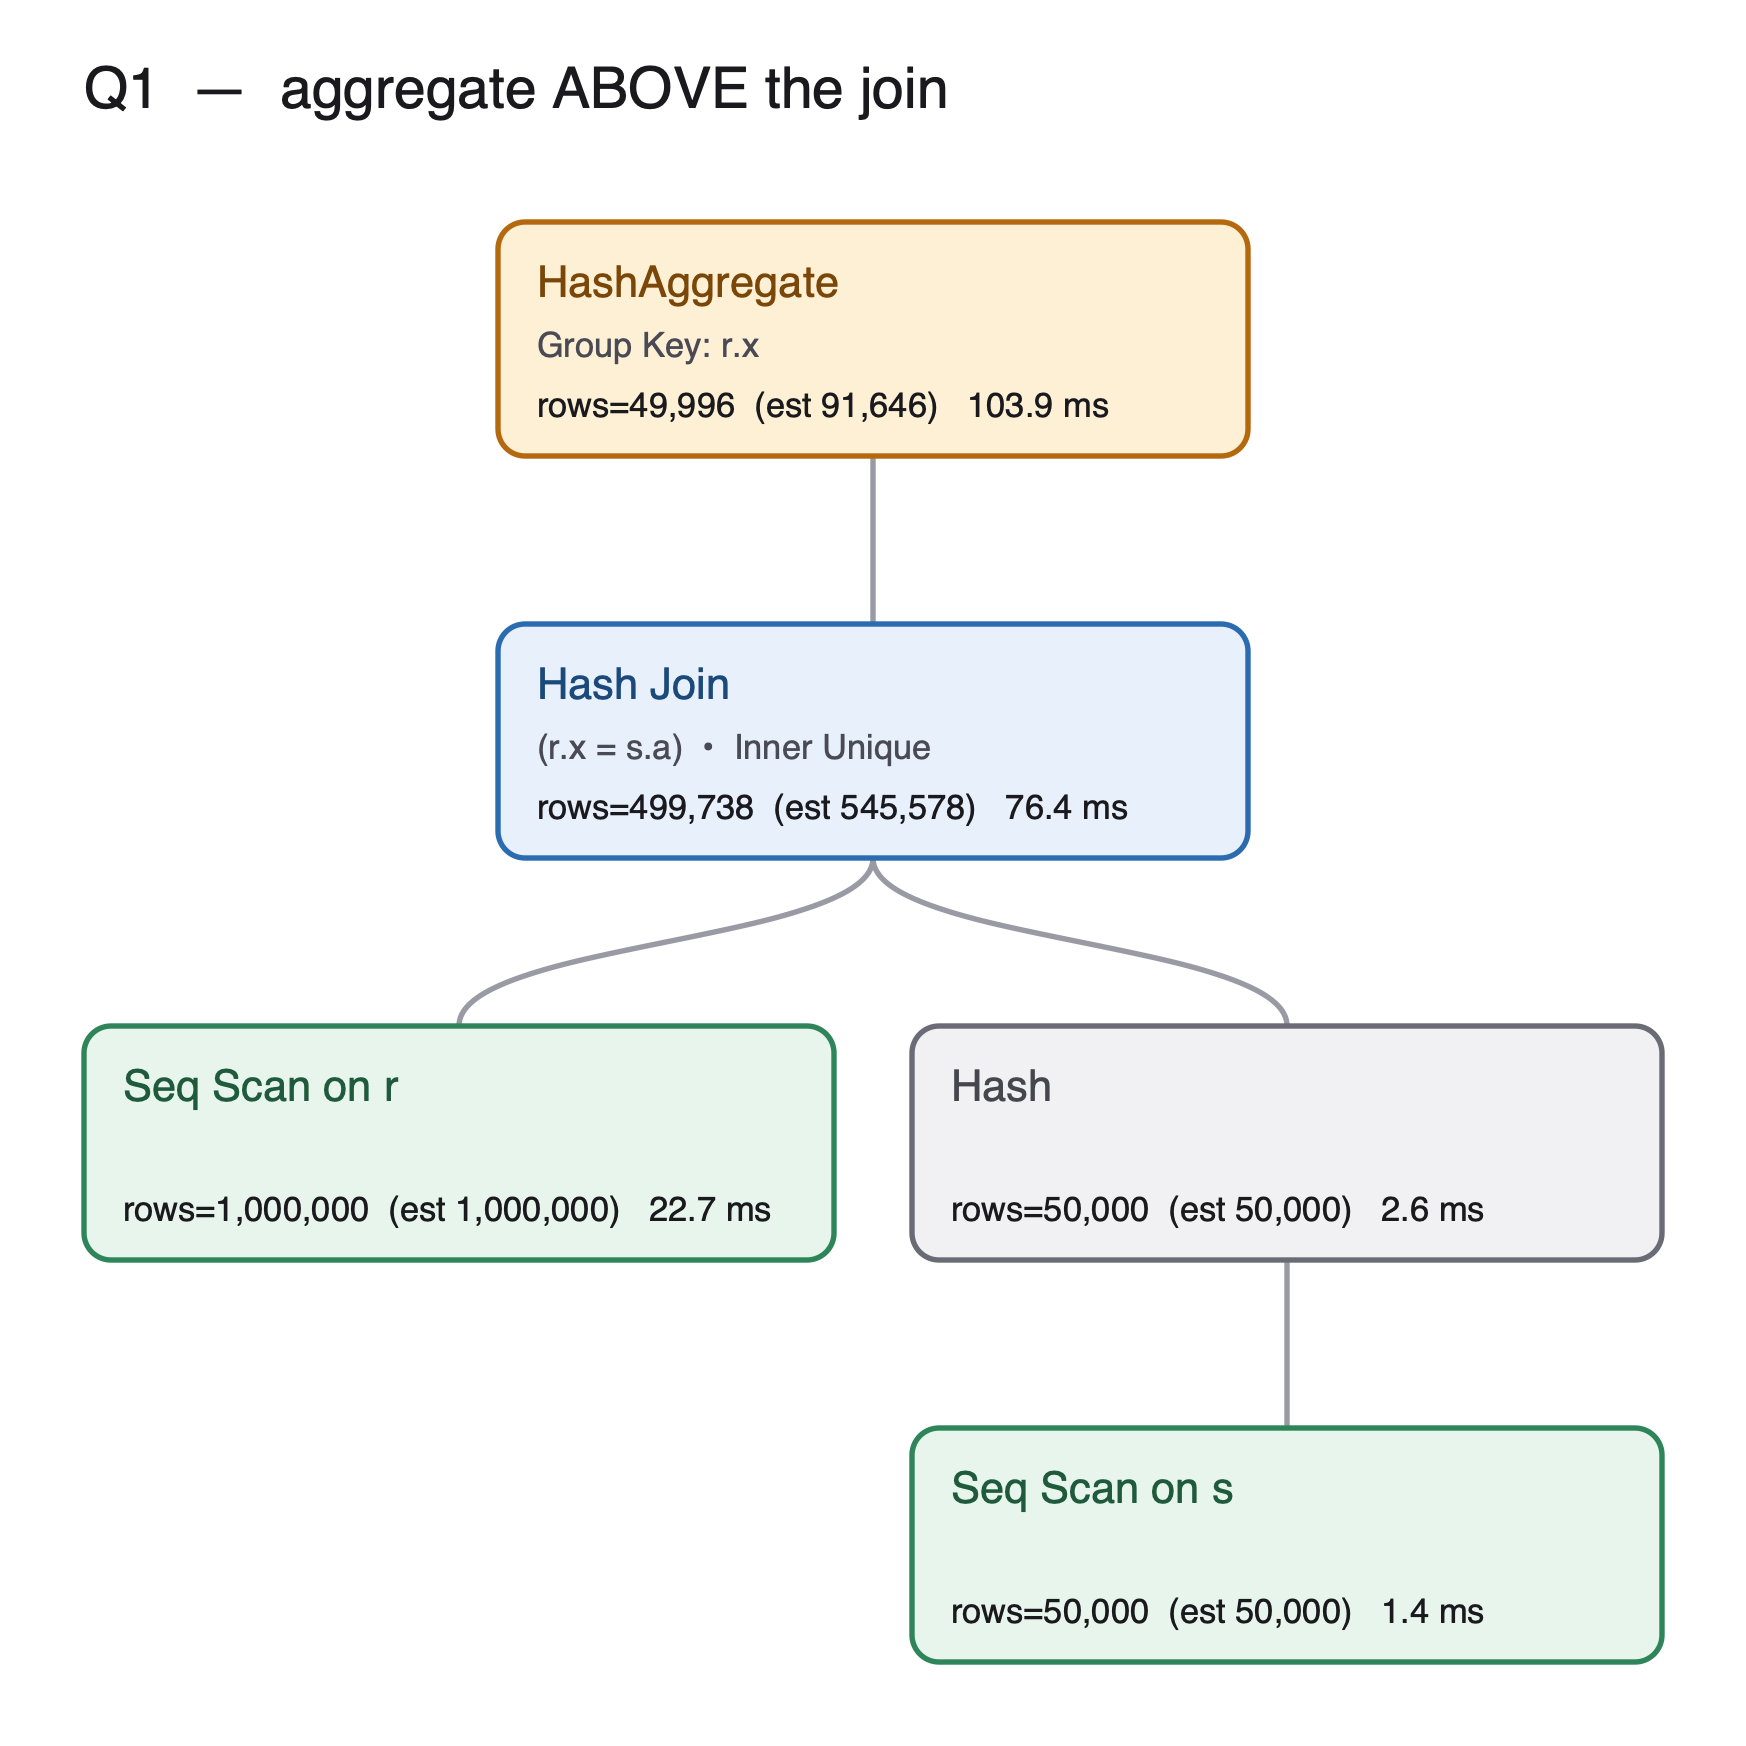
\includegraphics[width=0.47\linewidth]{figs/q1_plan.png}\hfill
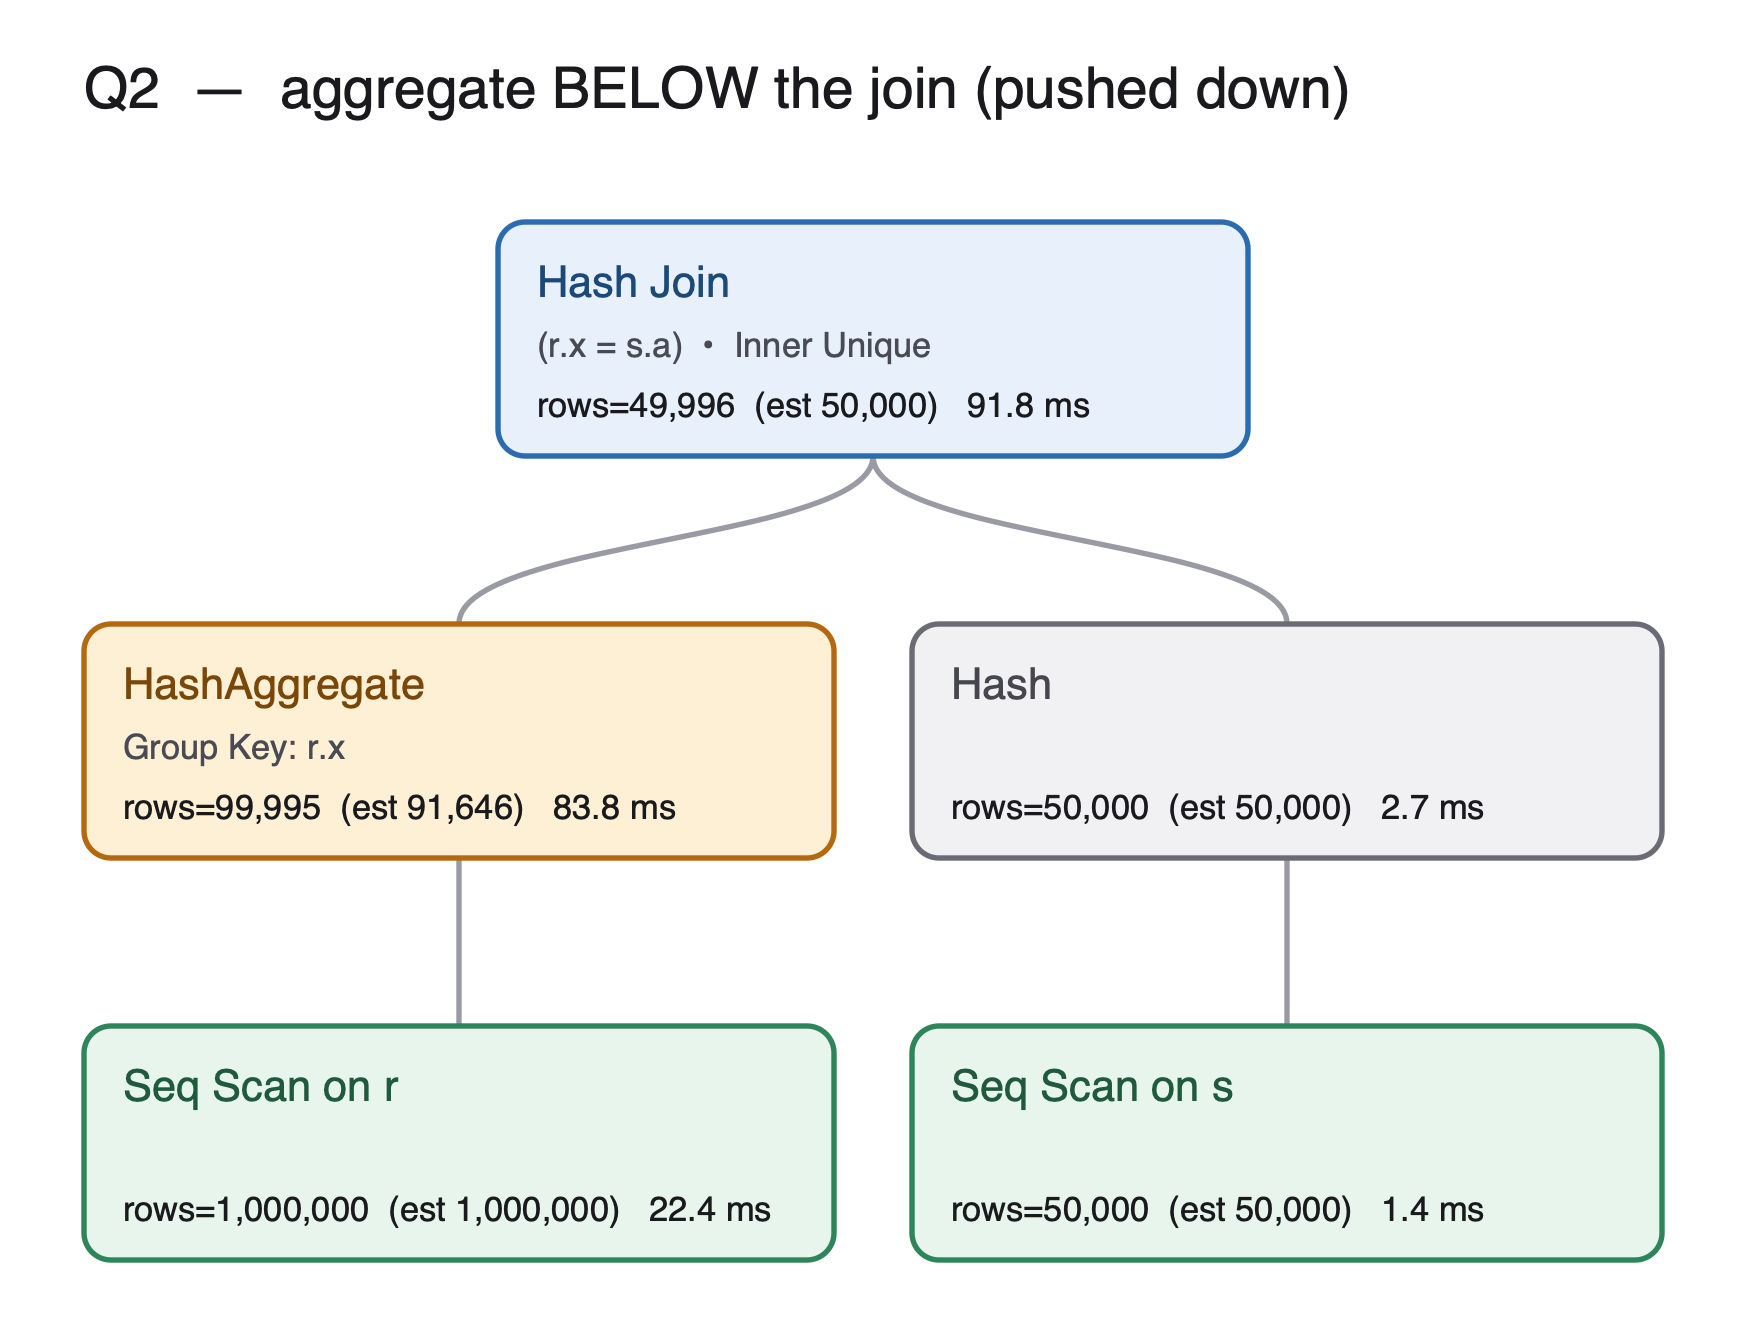
\includegraphics[width=0.47\linewidth]{figs/q2_plan.png}
\caption{PostgreSQL 18 \texttt{EXPLAIN (ANALYZE, VERBOSE, BUFFERS)} for $Q_1$ (left) and
$Q_2$ (right). Note \texttt{Inner Unique} on both joins: the planner read the primary key
and recorded ``at most one match on the inner side''. \emph{That flag is the same fact the
provers write as $\sq{S(a)}$} --- Postgres uses it to stop probing early, the provers use
it to justify the rewrite.}
\label{fig:pgplans}
\end{figure}

\begin{table}[h]\centering\small
\begin{tabular}{@{}lrr@{}}
\toprule
 & $Q_1$ (agg above) & $Q_2$ (agg below)\\
\midrule
rows entering the aggregate & 499{,}738 & 1{,}000{,}000\\
groups produced             & 49{,}996  & 99{,}995\\
rows entering the join      & 1{,}000{,}000 & 99{,}995\\
final rows                  & 49{,}996  & 49{,}996\\
execution time              & 105.5\,ms & 93.1\,ms\\
\bottomrule
\end{tabular}
\caption{Measured. The pushdown is only $\approx$12\% faster here and its aggregate does
\emph{more} work; the win comes from the join seeing 99{,}995 rows instead of $10^6$.
Whether to apply the rewrite is a cost question --- entirely separate from whether it is
\emph{correct}, which is what this document is about.}
\end{table}

\subsubsection{Why the primary key is load-bearing}
\label{sec:pkcounter}

Give $S$ a duplicate ($a=1$ twice, no key) and run the same two queries on the same $R$:

\begin{center}\small
\begin{tabular}{@{}lll@{}}
\toprule
 & result & rows\\\midrule
$Q_1$ (agg above join) & $(1,\,60)$ & 1\\
$Q_2$ (agg below join) & $(1,\,30),\ (1,\,30)$ & 2\\
\bottomrule
\end{tabular}
\end{center}

Not equivalent, and wrong in two independent ways:

\begin{itemize}
\item $Q_1$ joins first, so every $R$ row is duplicated \emph{before} the aggregate sees
      it. The bag entering \lstinline|SUM| becomes $\{10,10,20,20\}$ instead of
      $\{10,20\}$, so the \textbf{value} is corrupted: $60$ instead of $30$.
\item $Q_2$ aggregates first, so \lstinline|SUM| sees the clean bag. The duplication hits
      the \textbf{output row count} instead: two copies of $(1,30)$.
\end{itemize}

This is the same phenomenon Calcite compensated for in \S\ref{sec:calcite-fires}: with
$\mathrm{count} = 2$, Calcite's rewritten plan computes $30 \times 2 = 60$, matching $Q_1$.
On PostgreSQL, \texttt{Inner Unique} disappears from $Q_1$'s plan the moment the key is
dropped.

\keybox{The specification of the running example}{%
$Q_1 \equiv Q_2$ \textbf{if and only if} the join column on the right is distinct.
A prover that cannot turn ``\texttt{a} is a primary key'' into a usable algebraic fact
cannot prove this rewrite; one that proves it \emph{without} using the key is unsound.}
